\documentclass{aamas2010_cameraReady}
\usepackage{amsmath}

\pdfpagewidth=8.5truein
\pdfpageheight=11truein

\renewcommand\floatpagefraction{.9}
\renewcommand\topfraction{.9}
\renewcommand\bottomfraction{.9}
\renewcommand\textfraction{.1}   
\setcounter{totalnumber}{50}
\setcounter{topnumber}{50}
\setcounter{bottomnumber}{50}

\newcommand\bump{\vspace{10in}}

\usepackage{url}
\begin{document}

% In the original styles from ACM, you would have needed to
% add meta-info here. This is not necessary for AAMAS 2010 as
% the complete copyright information is generated by the cls-files.

% For appropriate information about authors and title written in the
% copyright information, you must use these commands. Note that the copyright
% box is not required for the initial submission.

\AuthorsForCitationInfo{Anonymous}
%\AuthorsForCitationInfo{Sean Luke, Vittorio Amos Ziparo}


\TitleForCitationInfo{Learn to Behave! Rapid Training of Behavior Automata}

\title{Learn to Behave!\\Rapid Training of Behavior Automata}

\sloppy

%\numberofauthors{2}

%\author{
%\alignauthor
%Sean Luke\\
%       \affaddr{Department of Computer Science}\\
%       \affaddr{George Mason University}\\
%       \affaddr{4400 University Drive MSN 4A5}\\
%       \affaddr{Fairfax, VA 22030 USA}\\
%       \email{sean@cs.gmu.edu}
%% 2nd. author
%\alignauthor
%Vittorio Amos Ziparo\\
%       \affaddr{Dipartimento di Informatica e Sistemistica}\\
%       \affaddr{Universit{\`a} di Roma ``La Sapienza''}\\
%       \affaddr{Via Ariosto 25, I-00185}\\
%       \affaddr{Rome, ITALY}\\
%       \email{ziparo@dis.uniroma1.it}
%}

%%%% IMPORTANT NOTE FROM SEAN
%%%% When de-anonymizing, see the example.tex file which also has something that has to be
%%%% uncommented as well. REMINDER.

\numberofauthors{1}
\author{
\alignauthor
By Anonymous\\
       \affaddr{~}\\
       \affaddr{ ~}\\
       \affaddr{~ }\\
       \affaddr{~ }\\
       \email{ ~}\\
}

\maketitle

\begin{abstract}
Programming robot or virtual agent behaviors can be a challenging task, and makes attractive the prospect of automatically learning the behaviors from the actions of a human demonstrator.  However, learning complex behaviors rapidly from a demonstrator may be difficult if they demand a large number of training samples.  We describe an architecture for rapid learning of recurrent behaviors from demonstration.  The architecture is based on deterministic hierarchical finite-state automata (HFAs) with classification algorithms taking the place of the state transition function.  This architecture allows for task decomposition, statefulness, parameterized features and behaviors, per-behavior feature set customization, and storage of learned behaviors in libraries to be used later on as elements in more complex behaviors.  We describe the system, then illustrate its application in a simple, but nontrivial,  foraging task involving multiple behaviors.

\end{abstract}

% Note that the category section should be completed after reference to the ACM Computing Classification Scheme available at
% http://www.acm.org/about/class/1998/.

\category{I.2.6}{Artificial Intelligence}{Learning}

%A category including the fourth, optional field follows...
%\category{D.2.8}{Software Engineering}{Metrics}[complexity measures, performance measures]

%General terms should be selected from the following 16 terms: Algorithms, Management, Measurement, Documentation, Performance, Design, Economics, Reliability, Experimentation, Security, Human Factors, Standardization, Languages, Theory, Legal Aspects, Verification.

\terms{Algorithms, Design, Human Factors}

%Keywords are your own choice of terms you would like the paper to be indexed by.

\keywords{Learning from Demonstration, Hierarchical Finite-state Automata, Agents, Robotics}

\section{Introduction}

Our goal is to enable the rapid, real-time training of complex, stateful agent behaviors.  Agent behavior training has applications in a variety of fields, including 3D animation, game level design, and autonomous robotics.  In these areas, programming custom domain-specific behaviors on-the-fly may not be desirable or possible, and so it is attractive to instead have the agent learn them from a trainer.

One of the challenges facing training, however, is the conflict between the real-time nature of training and the large numbers of samples that may be demanded by a challenging, high-dimensional domain.  It may not be feasible to ask a trainer to perform hundreds of trials to satisfy the needs of a learning algorithm.  Thus, one of our goals is to develop methods to reduce domain complexity, and ideally reduce the number of necessary samples, while not sacrificing the gamut of learnable behaviors.  We do this by taking advantage of domain knowledge in various ways, and thus our method lies somewhere in the middle-ground between explicit programming (that is, specification) and full, unfettered learning.

Our learned agent behaviors take the form of deterministic hierarchical finite-state automata (HFA).  The motivation underlying this choice is twofold. First, HFA are a widely adopted tool for modeling agent and robot behaviors, yet are simple enough to allow the demonstration of our learning approach.  Second, we chose HFAs as they enabled us to do task decomposition.

There are many HFA formulations.  Ours is straightforward: a learned behavior is a standard Moore Machine finite-state automaton, where each state is associated with a certain behavior, and also with a transition function which stipulates, given the current world situation, which state to transition to in the next time step.  There is a start state but no accepting states.  

%A state's behavior can either be a basic behavior hard-coded into the agent itself; or the behavior may itself be another, lower-level finite-state automaton.  In the second case, when in a state \(S\) associated with a lower-level finite-state automaton behavior \(B\), the agent performs the behaviors, and appropriate transitions, of \(B\) until such time that some world condition causes a transition away from \(S\) and to a new higher-level state \(S'\).  At this point \(B\)'s FSA is eliminated and the agent moves on to performing \(S'\).  The HFA may have any number of levels of embedded automata, but recursion is not permitted.

Our approach is to build an HFA iteratively: we allow the user to easily create an HFA based on a current library of behaviors (some of which may themselves be HFAs).  When the HFA is complete, it is added to the library to help build a more complex higher-level HFA.   One can create of course an HFA by coding it by hand: but of interest to us is the ability to {\it learn} the HFA by watching a demonstrator manipulate the agent.  As the agent moves about in the environment, the demonstrator directs it to perform various behaviors (and thus to transition to various new states). Each time the demonstrator requests such a transition, the system records the transition and the current world situation.
% (the feature vector provided the agent).  
At the end of the training period, from these records the system builds, for each state (behavior), a learned transition function indicating under what conditions the agent should transition to new states.  This is essentially a supervised learning task and can employ a variety classification algorithms: at present our learned models take the form of decision trees.

The learning domain for an HFA behavior can obviously be complex and of high dimension, depending on the number of basic behaviors and the dimensionality of the agent's feature vector.  This in turn can require a high number of training sessions to adequately describe the domain.  It is not reasonable to expect a demonstrator to perform that many training sessions, and so it is important to reduce the domain space complexity or training difficulty.  We have done this in three ways:

\begin{itemize}
\item An HFA encourages task decomposition.  Rather than learn one large behavior, the system may be trained on simpler behaviors, which are then composed into a higher-level learned behavior.  This essentially projects the full learning space into multiple lower-dimensional spaces.

\item Feature vector reduction.  Our system allows the user to specify precisely those features he feels are necessary for a given learned HFA, which in turn dramatically reduces the learning space.  Each HFA, including lower-level HFAs, may have its own reduced feature vector.

\item Generalization by parametrization.  All behaviors, including HFAs themselves, may be parameterized with {\it targets}: for example, rather than create a behavior \textsf{go-to-home-base}, we can create a general behavior \textsf{go-to(A)}, and allow for higher-level behaviors to specify the meaning of the target \textsf{A} at a future time.  This can significantly reduce the number of behaviors which must be trained.
\end{itemize}

By employing these complexity-reduction measures, our system ideally enables the rapid construction of complex behaviors, with internal state and a variety of sensor features, in real time entirely by training from demonstration.

The remainder of the paper is laid out as follows.  We begin with a discussion of related work.  We then describe the basic HFA model and our approach to learning the transition functions in the automaton.  We follow this with a training example of a nontrivial foraging behavior, then conclude with a discussion of future directions.

%Our automaton consists of a set \(\mathcal{S} = \{S_1, S_2, ..., S_n\}\) of {\it states}, exactly one of which is active at any time.  Each state corresponds to a {\it behavior} which the agent performs while that state is active.  The HFA also contains a set \(\mathcal{E} = \{E_1, E_2, ..., E_n\}\) of {\it transition edges}, where each edge \(E_i\) is a triple of the form \(\langle S, S', C\rangle\) indicating a current {\it outgoing} state \(S\), a new {\it incoming} state \(S'\), and a {\it condition} \(C\).  Edges control how the HFA transitions from state to state: if \(S\) is presently the active state, and the condition \(C\) occurs in the environment, and \(\langle S, S', C\rangle \in \mathcal{E}\), then the HFA will transition to \(S'\) as its new active state.  We presume that for a given state \(S\), all edges with \(S\) as their outgoing state have disjoint and non-conflicting conditions.  Furthermore we may describe all such edges collectively as a {\it transition function} \(T(S, C)\rightarrow S'\) which maps the current state \(S\) and the current world situation \(C\) into a transition to a new state \(S'\).  One state \(S_0\) is the {\it start state}.

%The finite-state automaton is hierarchical in the following way: the behaviors associated with a given state \(S\) may either be hard-coded {\it basic behaviors} built into the agent itself; or they may themselves be finite-state automata.  When we transition to \(S\), and it is associated with a FSA behavior, we initialize the 


%!TEX root = paper.tex

\section{Related Work}

Our approach generally fits under the category of {\it learning from demonstration} \cite{DBLP:conf/icml/AtkesonS97}, an overall term for training agent actions by having a human demonstrator perform the action on behalf of the agent.  Because the proper action to perform in a given situation is directly provided to the agent, this is broadly speaking a supervised learning task, though a significant body of research in the topic actually involves reinforcement learning, whereby the demonstrator's actions are converted into a reinforcement signal from which the agent is expected to derive a policy.  The lion's share of learning from demonstration literature comes not from virtual or game agents but from autonomous robotics.  For a large survey of the area, see \cite{argall2009}.

\paragraph*{Learning Plans}
One learning from demonstration area, closely related to our own research, involves the learning of largely directed acyclic graphs of behaviors (essentially plans) from sequences of actions \cite{DBLP:conf/atal/AngrosJRS02,DBLP:journals/tsmc/NicolescuM01,DBLP:conf/atal/NicolescuM03,DBLP:conf/hri/RybskiYSV07}, possibly augmented with sequence iteration \cite{DBLP:conf/iros/VeeraraghavanV08}.  Like our approach, these plans are often parameterizable.

Such plan networks generally have limited or no recurrence: instead they usually tend to be organized as sequences or simultaneous groups of behaviors which activate further behaviors downstream.  This is mostly a feature of the problem being tackled: such plans are largely induced from ordered sequences of actions intended to produce a result.  Since we are training goal-less behaviors rather than plans, our model instead assumes a rich level of recurrence: and for the same reason the specific ordering of actions is less helpful.

\paragraph*{Learning Policies}
Another large body of work in learning from demonstration involves observing a demonstrator perform various actions when in various world situations.  From this the system gleans a set of \(\langle\textit{situation, action}\rangle\) tuples performed and builds a policy function \(\pi(\textit{situation})\rightarrow\textit{action}\) from these tuples.   This can be tackled as a supervised learning task \cite{Bain96aframework,DBLP:journals/ras/BentivegnaAC04,DBLP:conf/hri/CalinonB07,dinerstein07,DBLP:journals/ras/KasperFSP01,DBLP:journals/ras/NakanishiMECSK04}.  However, some literature instead transforms the problem into a reinforcement learning task by providing the learner only with a reinforcement signal based on how closely the learned policy matches the tuples provided by the demonstrator \cite{DBLP:journals/cacm/CoatesAN09,yasutake2}.

Our approach differs from these methods in an important way.  Instead of learning {\it situation\(\rightarrow\)action} rules, our model learns the transition functions of an HFA with predefined internal states, each corresponding to a possible basic behavior.  This enables the demonstrator to differentiate transitions to new behaviors not just based on the current world situation but also the current behavior.  Another, somewhat different use of internal state would be to distinguish between aliased observations of hidden world situations, something which may be accomplished through learning hidden Markov models (for example, \cite{4756000}).


\paragraph*{Hierarchical Models}
The use of hierarchies in robot or agent behaviors is very old indeed, going back as early as Brooks's Subsumption Architecture \cite{brooks}.  Hierarchies are a natural way to achieve layered learning \cite{DBLP:conf/ecml/StoneV00} via task decomposition.  This is a common strategy to simplify the state space: see \cite{4354062} for an example.  While it is possible in these cases to induce the hierarchy itself, usually such methods iteratively compose hierarchies in a bottom-up fashion.

Our HFA model bears some similarity to hierarchical behavior networks such as those for virtual agents \cite{Bindiganavale00dynamicallyaltering} or physical robots \cite{DBLP:conf/atal/NicolescuM02}, in which feed-forward plans are developed, then incorporated as subunits in larger and more complex plans.  In such literature, the actual application of hierarchy to learning from demonstration has been unexpectedly limited.  However, learning from demonstration has been applied more extensively to multi-level reinforcement learning, as in \cite{yasutake1}, albeit with a fixed hierarchy.

\paragraph*{Language Induction}
One cannot mention learning finite state automata without noting that they have a long history in language induction and grammatical inference, with a correspondingly massive literature.  For recent surveys of techniques using automata for grammar induction, see \cite{Parekh00grammarinference, vidal}.  However the goal of this literature is fundamentally different from ours in this paper.  Specifically, in language induction, the learning algorithm is given a set of positive and negative string examples and generates an automaton which induces an underlying language.  Typically these algorithms make no assumptions about the number of states, assume the states are unlabelled, typically assume a small set of transition conditions, and include accepting or rejecting states.  In contrast we are not interested in terminating automata, and seek to induce only the edges among a prespecified set of labeled states, given examples with labelled transitions from state to state.

%!TEX root = paper.tex


\section{The HFA Model}

Using our system, a trainer iteratively develops new finite-state automata, whose states encompass behaviors drawn from a behavior library.  An automaton is learned by observing the trainer as he selects various behaviors in various situations.  Once learned, the automaton can then be added as a behavior in the library, and then may be itself used as a state in more complex automata.  In the following, we first describe the hierarchical finite state automaton model, and in the next section we detail our approach for learning the automaton by demonstration from the trainer. 

%Our goal is to learn agent models based on a finite set of atomic behaviors ${\cal B}=\{b_{1},\ldots,b_{n}\}$ and a finite set of features ${\cal F}=\{f_{1},\ldots,f_{n}\}$. Behaviors correspond to pre-implemented actions to which the agent has access in order to build more complex behaviors, while features correspond to the perceptions used for modeling the state of the environment. 


%\subsection{The HFA Model}




\begin{figure}[t]
\begin{center}
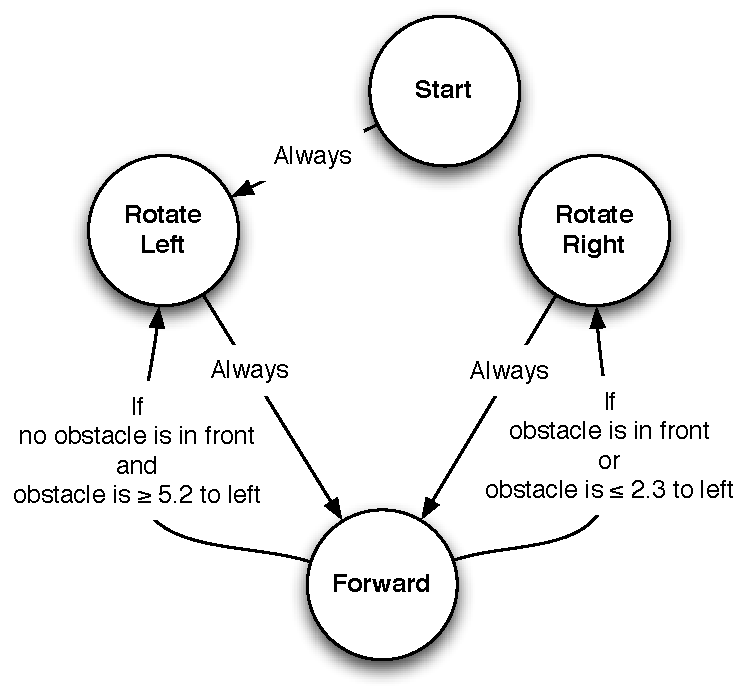
\includegraphics[width=3in]{WallFollower.pdf}
\end{center}
\caption{A simple finite-state automaton for wall following (counter-clockwise).  All conditions not shown are assumed to indicate that the agent remain in its current state.}
\label{fsa}
\end{figure}


\paragraph*{States and Behaviors}
Our HFAs model Moore machines: that is, each state corresponds to a behavior, and when in a state, the HFA performs that behavior.  A behavior may be an atomic behavior or may itself be another HFA, leading to the hierarchical definition of the model.  Atomic behaviors are hard-coded behaviors provided by the system.  For example, the behavior \textsf{rotate-left} might be a basic behavior: when employing this behavior, the agent will spin counterclockwise at some rate.  The HFA always begins in the {\it start state} (\textsf{start}), associated with a special \textsf{idle} behavior, and which always transitions immediately to some other state.  Another special state is the optional {\it done state}, whose behavior simply sets a ``done'' flag and immediately transitions to the start state.  This is used to potentially indicate to higher-level HFAs that the behavior of the current HFA is ``done''.  

 Figure \ref{fsa} shows a simple automaton with four states, corresponding to the behaviors \textsf{start}, \textsf{rotate-left}, \textsf{rotate-right}, and \textsf{forward}.  It may appear at first glance that not all HFAs can be built with this model: for example, what if there were {\it two} states in which the \textsf{rotate-left} behavior needed to be done?  This can be handled by creating a simple HFA which does nothing but transition to the \textsf{rotate-left} state and stay there.  This automaton is then stored as a behavior called \textsf{rotate-left2} and used in our HFA as an additional state, but one which performs the identical behavior to \textsf{rotate-left}. 

\paragraph*{Features}
Transitions from state to state are triggered by observable {\it features} of the environment. One such feature might be \textsf{distance-to-closest-obstacle-on-my-left}.  At any time, this feature yields a non-negative value indicating the distance to such an obstacle.   In our system features presently take three forms: {\it categorical features}, which return unordered values like ``red'' or ``blue'';  {\it continuous features}, which return real-valued numbers (like distances); and {\it toroidal features}, which return real-valued numbers but which are assumed to wrap around in a toroidal fashion (like angles).  Boolean features are typically modeled as categorical features.  One special boolean feature is the \textsf{done} feature, which is true if the current behavior is a lower-level HFA, and if it has triggered its \textsf{done} flag.

\paragraph*{Targets}
Importantly, our approach supports parameterized, general-purpose behaviors and transitions.  Rather than create a behavior called \textsf{go-to-obstacle-number-42}, we can create a behavior called \textsf{go-to(A)}, where \textsf{A} may be specified later.  Similarly, rather than the aforementioned feature \textsf{distance-to-closest-obstacle-on-my-left}, we might instead have the more general feature \textsf{distance-to(B)}.  Thus, this separate notion of features and behaviors from the {\it targets} to which they apply.  For example, a feature or behavior may be either specified with regard to one or more {\it ground targets} (``obstacle 42'' or ``the closest obstacle on my left'')\,---\,resulting in a behavior such as \textsf{go-to}(\textsf{obstacle-42})\,---\,or the target may simply be left unspecified (\textsf{A}), to be bound to a ground target at some later time.  In the latter case, the unbound target is called a {\it parameter}.

When an HFA employs features or behaviors with as-of-yet unbound targets (parameters), it must itself present those parameters when used as a behavior by some higher-level HFA.  Thus HFAs themselves may be parameterized.

%Additionally, when an FSA behavior is created, all parameters of features and behaviors within the FSA must be either bound to ground targets or bound to the FSA's own parameters.  In the latter case the FSA behavior itself becomes a parameterized behavior.

\paragraph*{Transitions}  In traditional finite-state automata, transitions are represented by directed edges between nodes, each labelled with a condition which may or may not be true about the current features of the environment.  Without loss of generality, it's more useful for us to think of a {\it transition function} which maps the current state and the current feature vector into a new state.  The start state always transitions to a specific other state; and the done state always transitions to the start state. 


%Rules are based  on a finite set of features ${\cal F}=\{f_{1},\ldots,f_{n}\}$ that correspond to the perceptions used for modeling the state of the environment.  
%Node transitions take the form of rules which are or are not true about the environment.  We presume that all transitions leaving a node constitute a set of disjoint rules.  If no such rule is true, no transition is triggered and the FSA stays in its present state.  For example, were our FSA presently in the {\it forward} behavior (moving forward), and an obstacle was in front or less than $2.3$ units to the left, we would transition to the {\it rotate right} behavior and start rotating to the right.  On the other hand, if no obstacle was in front and an obstacle was further than $5.2$ units to the left, we would transition to the {\it rotate left} behavior.  Finally, if neither of these were true, we would continue moving forward.  All transitions leaving a given state are collectively embodied in a single {\bf transition} object associated with that state: thus an FSA behavior with \(N\) states also has \(N\) transition objects.  

\paragraph*{Operating the HFA}

Each timestep the HFA is advanced one tick: it performs one step of the behavior associated with its current state, then applies the transition function to determine a new state for next timestep, if any.  When a performed behavior is itself an HFA, this operation is recursive: the child HFA likewise performs one step of {\it its} current behavior, and applies {\it its} transition function.  Additionally, when an HFA transitions to a state whose behavior is an HFA, that HFA is initialized: its initial state is set to the start state, and its ``done'' flag is cleared.

\paragraph*{Formal Model}
 For the purposes of this work, we define the class of hierarchical finite-state automata models  $\cal H$ as the set of tuples \( \langle \mathcal{S}, \mathcal{F}, T, \mathcal{B}, M \rangle\) where:
\begin{itemize}
\item $\mathcal{S} = \{S_0, S_1, \ldots, S_n\}$ is a set of {\it states}, including a distinguished start state $S_{0}$, and possibly also one ``done'' state \(S_*\).  Exactly one state is active at any time.

\item ${\cal F}=\{F_1,F_{2}, \ldots,F_{n}\}$ is a set of  {\it observable features} in the environment. The set of features is partitioned in three disjoint subsets representing categorical (${\cal C}$), continuous (${\cal R}$) and toroidal (${\cal A}$) features. Each $F_{i}$ can assume a value $f_{i}$ drawn from a finite (in the case of ${\cal C}$) or infinite (in the case of ${\cal R}$ and ${\cal A}$) number of possible values.  At any point in time, the present assumed values \(\vec f = \langle f_1, f_2, \ldots, f_n\rangle\) for each of the \(F_1, F_2, \ldots, F_n\) are known as the environment's current {\it feature vector}.

\item \(T: F_1 \times F_2 \times \ldots \times F_n \times \mathcal S \rightarrow \mathcal S\) is a {\it transition function} which maps a given state \(S_i\), and the current feature vector  \(\langle f_1, f_2, \ldots, f_n\rangle\), onto a new state \(S_j\).  The start state and done state have unilateral transitions:  \(\exists S_{k\neq0} \forall \vec f: T(\vec f, S_0) = S_k\), $\forall S_{k} \neq S_{*}\; \forall {\vec f}\; T(\vec f,S_{k})\neq S_{0}$ and \(\forall \vec f: T(\vec f, S_{*}) = S_0\).

%where each edge \(E_i\) is a triple of the form \(\langle S, S', C\rangle\) indicating a current {\it outgoing} state \(S\), a new {\it incoming} state \(S'\), and a {\it condition} \(C\). A {\it condition} \(C\) can be any propositional formula, where propositions  take the form of:
%\begin{itemize}
%\item   $F_{i}=cat$, where $F_{i}\in  {\cal C}$ and $cat$ is a  category of $f$ 
%\item   $F_{i}<v$, where $F_{i}\in  {\cal R}$ and $v \in \mathbb{R}$
%\item   $v_{1}\leq F_{i} <v_{2}$, where $F_{i}\in  {\cal T}$ and $v_1,v_{2} \in \mathbb{R}$
%\end{itemize}

\item ${\cal B}=\{B_1,B_{2},\ldots,B_{n}\}$ is a set of {\it atomic behaviors}.   By default, the special behavior {\sf idle}, which corresponds to inactivity, is in ${\cal B}$, as may also be the optional behavior {\sf done}.

\item \(M: \mathcal{S}\rightarrow {\cal H} \cup {\cal B}\) is a one-to-one mapping function of states to basic behaviors or hierarchical automata.  $M(S_{0})= \textsf{idle}$, and \(M(S_{*})=\textsf{done}$.  \(M\) is constrained by the stipulation that recursion is not permitted, that is, if an HFA \(H\in\cal H\) contains a mapping \(M\) which maps to (among other things) a child HFA \(H'\), then neither \(H'\) nor any of its descendent HFAs may contain mappings which include \(H\).  
\end{itemize}

%A condition can be evaluated over a set of feature values $\langle f_1,\ldots,f_{n}\rangle\in F_{1}\times \ldots \times F_{n}$, i.e. $C(\langle f_1,\ldots,f_{n}\rangle) \in \{\top,\bot\}$.

%\subsubsection*{Learning}
%We presume that for a given state \(S\), all edges with \(S\) as their outgoing state have disjoint and non-conflicting conditions.  Furthermore we may describe all such edges collectively as a {\it transition function} \(T: {\cal S}\times  F_{1}\times \ldots \times F_{n} \rightarrow {\cal S}\) defined as: 
%$$\forall\; S,S'\in{\cal S}\;\;\;\forall\;\langle f_1,\ldots,f_{n}\rangle\in F_{1}\times \ldots \times F_{n}$$ $$T(S,\langle f_1,\ldots,f_{n}\rangle)=S' \iff $$ $$\exists \; \langle S, S', C\rangle\in {\cal E} \mbox{ s.t. } C(\langle f_1,\ldots,f_{n}\rangle) \mbox{ is } true$$

%The learning task consists in learning the transition function $T$.

We further generalize the model by introducing free variables ($G_1,\ldots,G_{n}$) for basic behaviors and features: these free variables are known as {\it targets}.  The model remains unaltered, by replacing behaviors $B_{i}$ with $B_i(G_1,\ldots,G_{n})$ and features $F_{i}$ with $F_{i}(G_{1},\ldots,G_{n})$. The main differences are that the evaluation of the transition function and the execution of behaviors will both be based on ground instances of the free variables.


\section{Learning from Demonstration}

%\subsubsection*{Training}

The above mechanism is sufficient to hand-code HFA behaviors to do a variety of tasks; but our approach was meant instead to enable the learning of such tasks.  Our learning algorithm presumes that the HFA has a fixed set of states, comprising the combined set of atomic behaviors and all previously learned HFAs. Thus, the learning task consists only of learning the transitions among the states: given a state and a feature vector, decide which state (drawn from a finite set) to transition to.  This is an ordinary classification task.  Specifically, for each state \(S_i\) we must learn a classifier \(\vec f \rightarrow \cal S\) whose attributes are the environmental features and whose classes are the various states.  Once the classifiers have been learned, the HFA can then be added to our library of behaviors and itself be used as  a state later on.

Because the potential number of features can be very high, and many unrelated to the task, and because we want to learn based on a very small number of samples, we wish to reduce the dimensionality of the input space to the machine learning algorithm.  This is done by allowing the user to specify beforehand which features will matter to train a given behavior.  For example, to learn a Figure-8 pattern around two unspecified targets A and B, the user might indicate a desire to use only four parameterized features: \textsf{distance-to(A)}, \textsf{distance-to(B)}, \textsf{direction-to(A)}, and \textsf{direction-to(B)}.  During training the user temporarily binds A and B to some ground targets in the environment, but after training they are unbound again.  The resulting learned behavior will itself have two parameters (\textsf{A} and \textsf{B}), which must ultimately be bound to use it in any meaningful way later on.   

The training process works as follows.  The HFA starts in the ``start'' state (idling).  The user then directs the agent to perform various behaviors in the environment as time progresses.   When the agent is presently performing a behavior associated with a state \(S_i\) and the user chooses a new behavior associated with the state \(S_j\), the agent transitions to this new behavior and records an {\it example}, of the form \(\langle S_i, \vec{f}, S_j\rangle\), where \(\vec{f}\) is the current feature vector.  Immediately after the agent has transitioned to \(S_j\), it turns out to be often helpful to record an additional example of the form \(\langle S_j, \vec{f}, S_j\rangle\).  This adds at least one ``default'' (that is, ``keep doing state \(S_j\)'') example, and is nearly always correct since in that current world situation the user, who had just transitioned to \(S_j\) would nearly always want to stay in \(S_j\) rather than instantaneously transition away again.

At the completion of the training session, the system then builds transition functions from the recorded examples.  For each state \(S_k\), we build a decision tree \(D_{S_k}\) based on all examples where \(S_k\) is the first element, that is, of the form \(\langle S_k, \vec{f}, S_i\rangle\).  Here, \(\vec{f}\) and \(S_i\) form a data sample for the classifier: \(\vec{f}\) is the input feature and \(S_i\) is the desired output class.  If there are no examples at all (because the user never transitioned from \(S_k\)), the transition function is simply defined as always transitioning to back to \(S_k\).

At the end of this process, our approach has built some \(N\) decision trees, one per state, which collectively form the transition function for the HFA.  After training, some states will be unreachable because the user never visited them, and so no learned classification function ever mapped to them.  These states may be discarded.  The agent can then be left to wander about in the world on its own, using the resulting HFA.

%We note that equating behaviors with states is not sufficient for a general Moore-machine FSA: in a real Moore machine, multiple states may perform the same behavior.  Thus if there is only one ``go to A'' button, two states which require going to A will require special handling.  Our approach deals with this in one of two ways.  First, our approach might permit multiple buttons which do the same behavior (but which represent separate states in the FSA).  Second, it's straightforward to train a simple one-state FSA which simply does ``go to A''.  This FSA can then be named, say, ``go to A number 2'' and be included along with ``go to A'' for the user to use: they're different states (technically different behaviors) but ultimately do exactly the same thing.
%
%\paragraph{Toroidal Features -pie slice} We pause to note how we implemented toroidal features in decision trees.  Because angular regions are so common (and are toroidal), toroidal features are important.  The decision tree performs splits on toroidal regions much like it performs splits on continuous regions: by sorting the data by feature value and then finding the lowest-information split.  However whereas continuous splits involve finding a single split point \(A\) and breaking the examples into values \(< A\) versus \(\geq A\), toroidal splits instead involve finding {\it two} split points \(A\) and \(B\), with \(A < B\), and breaking the data into values \(v\) for which \(A \leq v < B\) and values which are either \(< A\) or \(\geq B\).  We term these groups ones which are ``inside'' and ``outside'' the split respectively.  We realize the cost of finding not one but two split values increases the computational complexity of finding an optimal split point by an additional \(O(n)\).  Though we doubt our approach here is original (and have not looked very hard), we have so far not found any other use of toroidal splits in the decision tree literature.

Though in theory many classification algorithms are applicable (such as K-Nearest-Neighbor or Support Vector Machines), in our experiments we chose to use a variant of the C4.5 Decision Tree algorithm~\cite{c4.5} for several reasons:
\begin{enumerate}
\item Many areas of interest in the feature space of our agent approximately take the form of rectangular regions (angles, distances, etc.).
\item Decision trees nicely handle various kinds of data: in our case, we used categorical, real-valued, and toroidal data (the latter requiring so-called ``pie-slice'' decision tree splits). 
\item Decision trees are particularly adept at handling unscaled dimensions in the feature space.  In our case, we would otherwise be faced with asking how many units of distance was equivalent to a degree of angle, or a change from ``true'' to ``false''.
\end{enumerate}

During the implementation and the evaluation of the decision tree learning algorithm, we found out that in some cases we would not want a deterministic classification. For example, when performing a wall-following behavior, we'd need to turn left some {\it percentage} of time. For this reason, we employed leaf nodes in the decision tree which yielded a probability distribution over classes rather than the single class typically generated through majority-value.
%!TEX root = paper.tex

\section{Example}

We have implemented an experimental research testbed for training agents using this approach (Figure \ref{horde}), written with the MASON multiagent simulation toolkit \cite{luke:simulation:2005}.
%%% Commented out for anonymity
%(see  {\sf http:/\!/cs.gmu.edu/\(\sim\)eclab/projects/mason/}).   
In the environment, our agent can sense a variety of things: the relative locations of obstacles, other agents of different classes, certain predefined waypoints, food locations, etc.  In this testbed, the experimenter trains an HFA by first selecting features relevant to the behaviors (see Figure \ref{features}), then grounding targets for behaviors and features, then directing the agent to perform behaviors by pressing various buttons or keystrokes, and then finally adding the trained HFA to the system library.



\begin{figure}[t]
\begin{center}
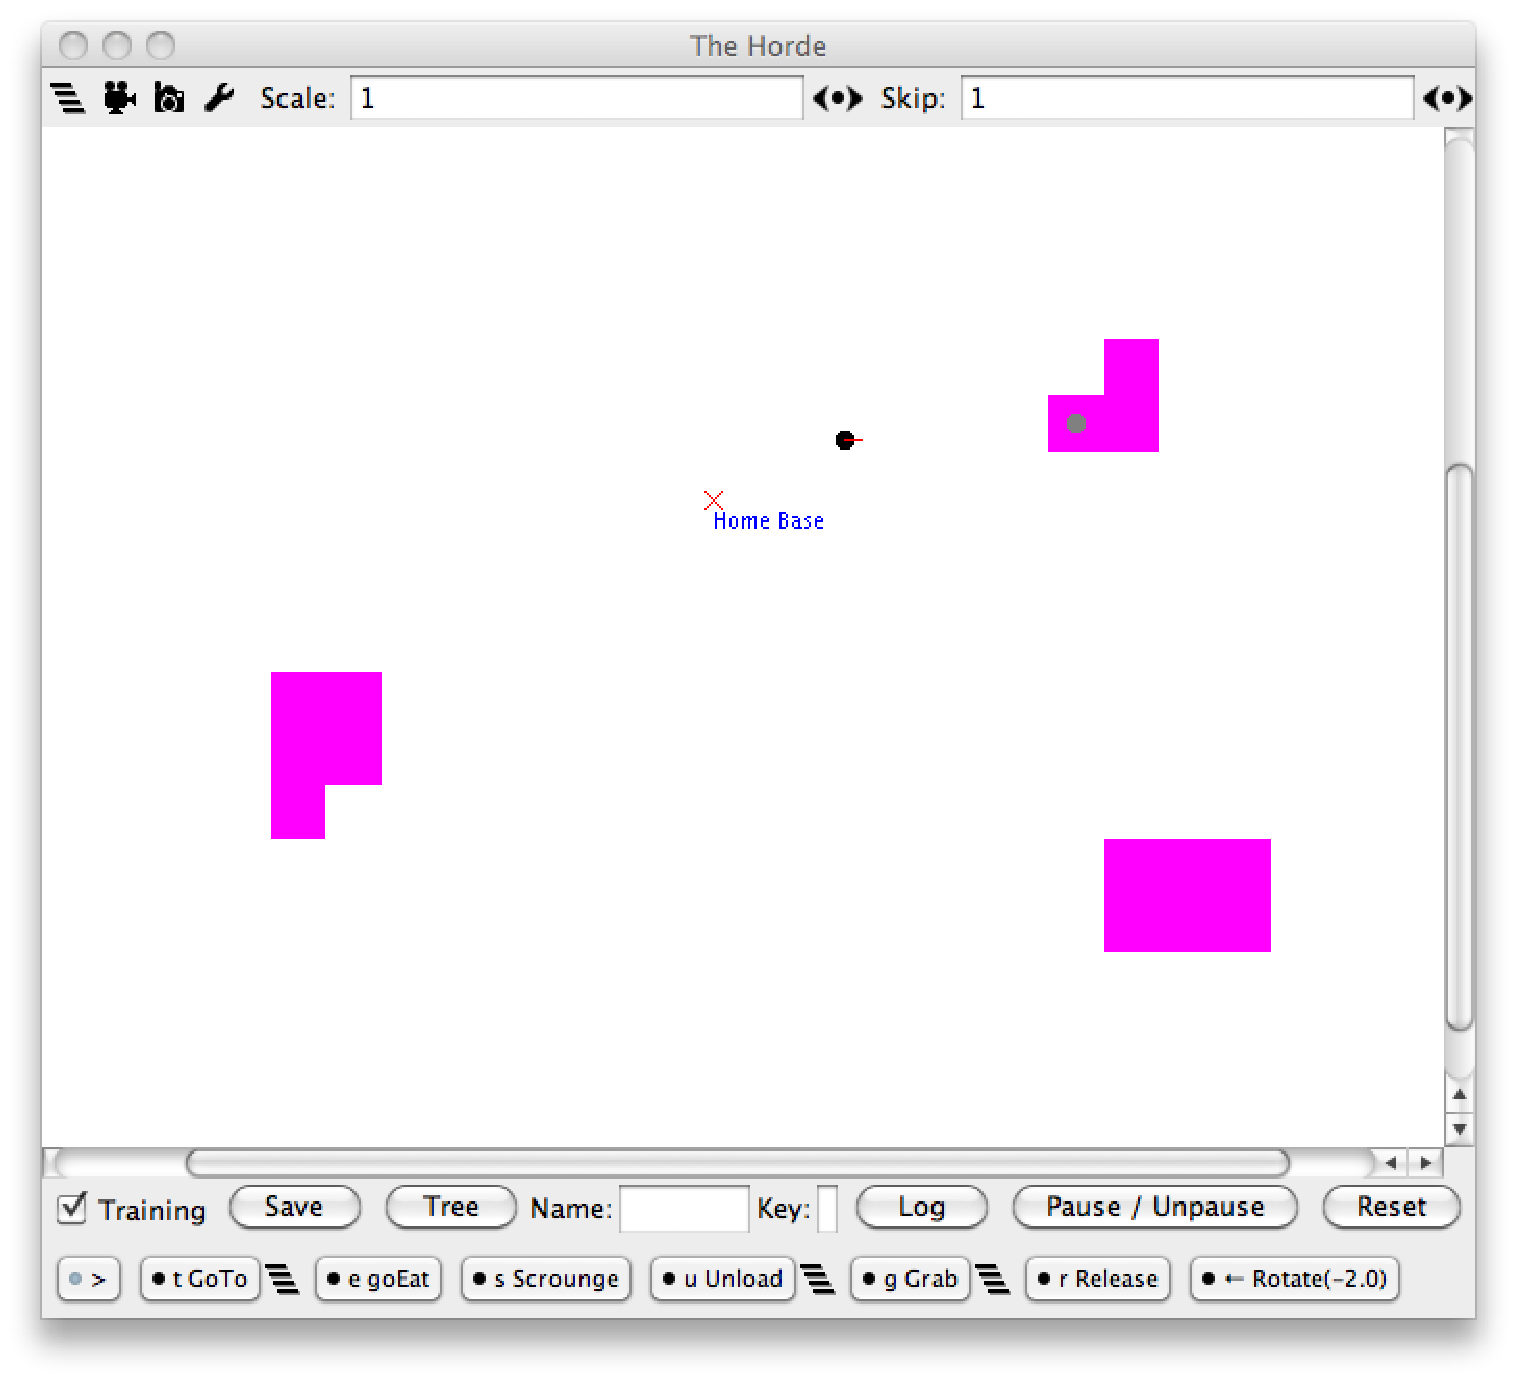
\includegraphics[width=3.3in]{ForagingHorde.pdf}
\end{center}
\caption{The foraging scenario in our testbed.}
\label{horde}
\end{figure}



We have successfully trained several simple behaviors, tracking and acquiring a target, wall-following, generic obstacle circumnavigation, and tracing paths (such as a figure eight path between two targets).  In this section,  we give an example where we have trained the agent to perform a moderately complex foraging task: to harvest food from food sources and bring it back to deposit at the agent's central station.  Food can be located anywhere, as can the station. Food at a given location can be in any concentration, and depletes, eventually to zero, as it is harvested by the agent.  The agent can only store so much food before it must return to the station to unload.  There are various corner cases: for example, if the agent depletes food at a harvest location before it is full, it must continue harvesting at another location rather than return to the station. The scenario is shown in Figure \ref{horde}: the black circle is the agent, pink areas are food sources, and the red ``\(\times\)'' (labelled ``Home Base'') is the station.

\begin{figure}[t]
\begin{center}
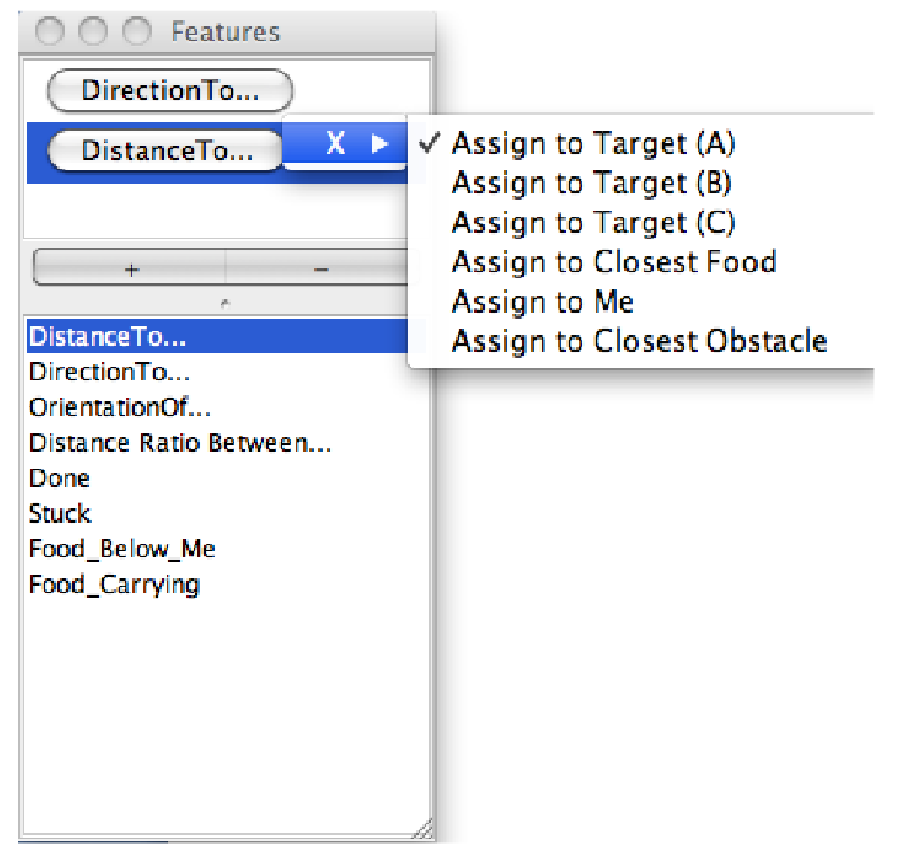
\includegraphics[width=2.5in]{Features.pdf}
\end{center}
\caption{Feature selection and target assignment.}
\label{features}
\end{figure}

\begin{figure*}[t]
\begin{center}
\noindent\begin{tabular}{cc}
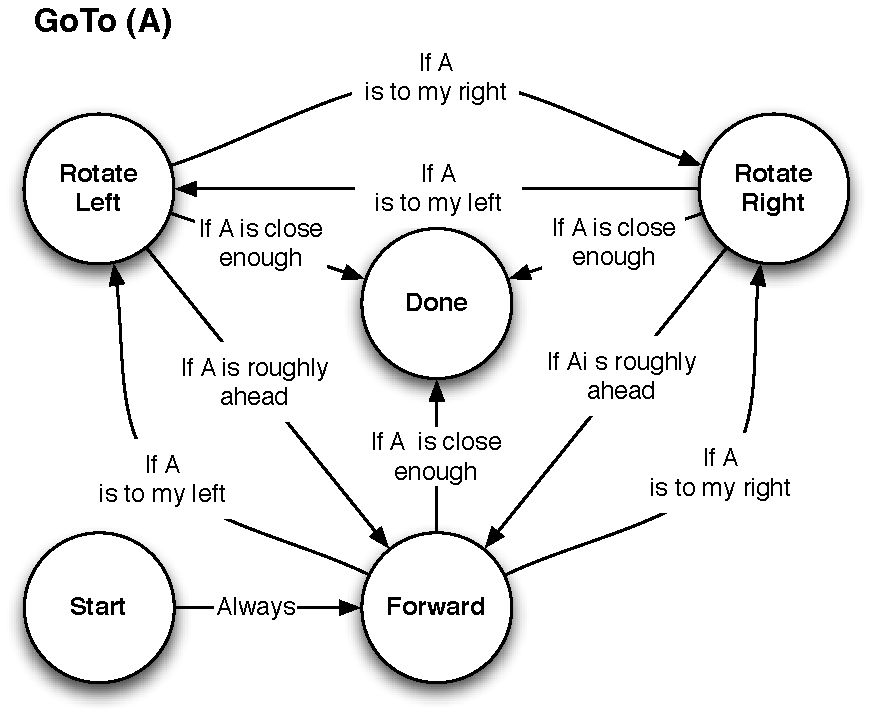
\includegraphics[width=3.5in]{GoTo.pdf}&
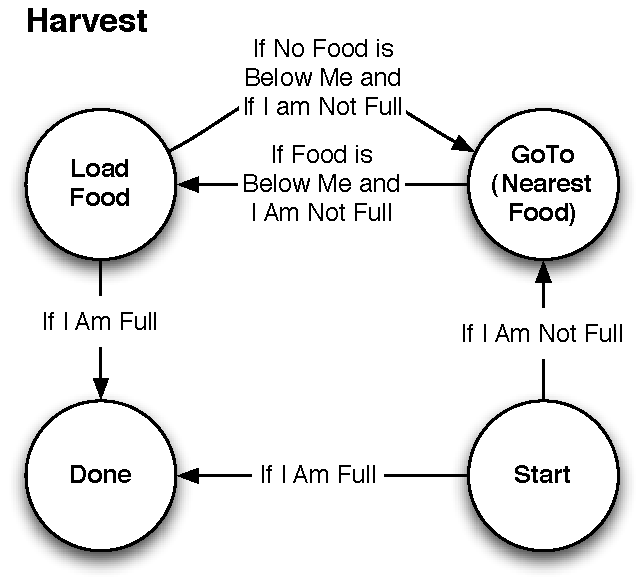
\includegraphics[width=2.6in]{Harvest.pdf}\\
\\
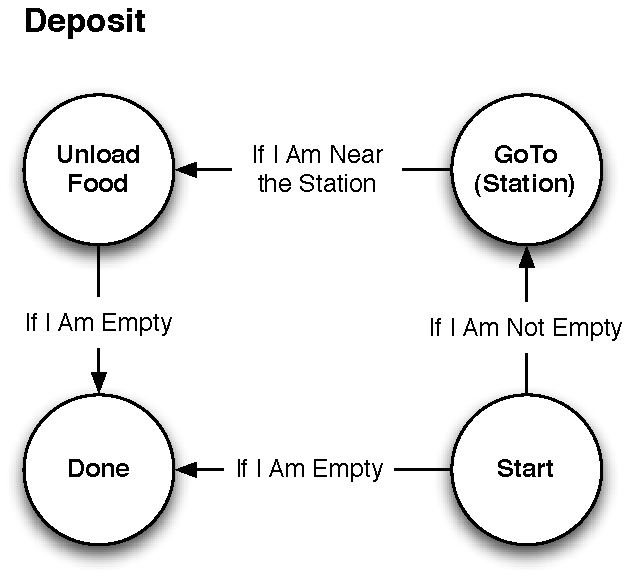
\includegraphics[width=2.6in]{Deposit.pdf}&
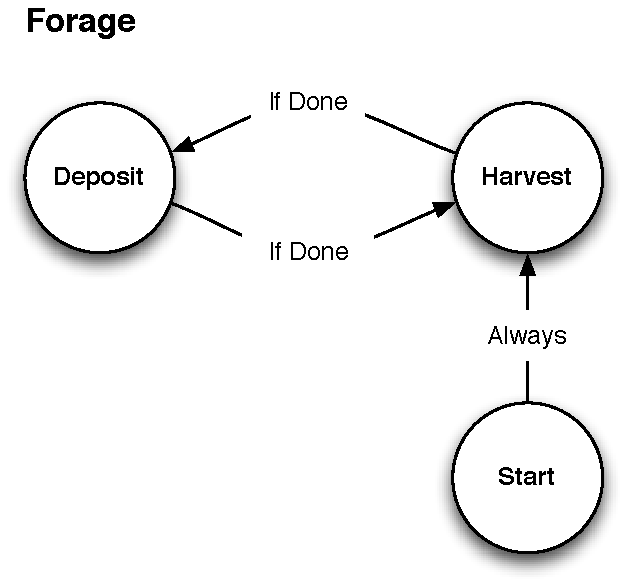
\includegraphics[width=2.6in]{Forage.pdf}\\
\end{tabular}
\end{center}
\caption{The Forage behavior and its sub-behaviors: Deposit, Harvest, and GoTo(\textit{Parameter} A).  All conditions not shown are assumed to indicate that the agent remain in its current state.}
\label{foraging}
\end{figure*}




Foraging tasks are of course old hat in robotics, and are not particularly difficult to code by hand.  But {\it training} such a behavior is less trivial.  We selected this task as an example because it illustrates a number of features special to our approach: our foraging behavior is in fact a three-layer HFA hierarchy; employs ``done'' states; involves real-valued, toroidal, and categorical (boolean) inputs; and requires one behavior with an unbound parameter used in two different ways.

The behavior is shown in Figure \ref{foraging}.  It requires seven basic behaviors: \textsf{start} and \textsf{done},  \textsf{forward}, \textsf{rotate-left}, \textsf{rotate-right}, \textsf{load-food} (deplete the current location's food by 1, and add 1 to the agent's stored food), and \textsf{unload-food} (remove all the agent's stored food).  It also requires several features: \textsf{distance-to(A)}, \textsf{angle-to(A)}, \textsf{food-below-me} (that is, how much food is located here), \textsf{food-stored-in-me}, and \textsf{done}.  Finally, it requires two targets to bind to A: the \textsf{station} and \textsf{nearest-food}.  

From this we decomposed the foraging task into a hierarchy of four HFA behaviors, and trained each one in turn as described next.  All told, we were able to train all four behaviors, and demonstrate the agent properly foraging, in a manner of minutes.

\paragraph*{The GoTo(A) Behavior} This behavior caused the agent to go to the object marked A.  The behavior was a straightforward bang-bang servoing controller: rotate left if A is to the left, else rotate right if A is to the right; else go forward; and when close enough to the target, enter the ``done'' state.
 
We trained the GoTo(A) behavior by temporarily declaring a marker in the environment to be Parameter A, and reducing the features to just \textsf{distance-to(A)} and \textsf{angle-to(A)}.  We then placed the agent in various situations with respect to Parameter A and ``drove'' it over to A by pressing keys corresponding to the \textsf{rotate-left}, \textsf{rotate-right}, \textsf{forward}, and \textsf{done} behaviors.  After a short training session, the system quickly learned the necessary behaviors to accurately go to the target and signal completion.  Once completed, it was made available in the library as \textsf{go-to(A)}.

\paragraph*{The Harvest Behavior} This behavior caused the agent to go to the nearest food, then load it into the agent.  When the agent had filled up, it would signal that it was done.  If the agent had not filled up yet but the food has been depleted, the agent would search for a new food location and continue harvesting.  This behavior employed the previously-learned \textsf{go-to(A)} behavior as a subsidiary behavior, binding its Parameter A to the \textsf{nearest-food} target.  This behavior also employed the features \textsf{food-below-me}, \textsf{food-stored-in-me}.

We trained the Harvest Behavior by directing the agent to go to the nearest food, then load it, then (if appropriate) signal ``done'', else go get more food.  We also placed the agent in various corner-case situations (such as if the agent started out already filled up with food).  Again, we were able to rapidly train the agent to perform harvesting.  Once completed, it was made available in the library as \textsf{harvest}.

\paragraph*{The Deposit Behavior} This behavior caused the agent to go to the station, unload its food, and signal that it is done.  If the agent was already empty when starting, it would immediately signal done.   This behavior also used the previously-learned \textsf{go-to(A)} behavior as a subsidiary state behavior, but instead bound its Parameter A to the \textsf{station} target.  It used the features \textsf{food-stored-in-me} and \textsf{distance-to(station)}.  We trained the Deposit Behavior in a similar manner as the Harvest Behavior, including various corner cases.  Once completed, it was made available in the library as \textsf{deposit}.

\paragraph*{The Forage Behavior} This simple top-level behavior just cycled between depositing and harvesting. Accordingly, this behavior employed the previously-learned \textsf{deposit} and \textsf{harvest} behaviors.  The behavior used only the \textsf{done} feature.

%!TEX root = paper.tex

\section{Conclusion}

In this paper, we have presented an approach for training agent behaviors using a hierarchical deterministic finite state automata model and a classification algorithm, implemented as a variant of the C4.5 algorithm. The main goal of our approach is to enable users to train agents rapidly based on a small number of training examples.  In order to achieve this goal, we trade off learning complexity with training effort, by enabling trainers to decompose the learning task in a hierarchical manner, to learn general parameterized behaviors, and to explicitly select the most appropriate features to use when learning. This in turn reduces the dimensionality of the learning problem. 

We have developed a proof of concept testbed simulator which appears to work well: we can train parameterized, hierarchical behaviors for a variety of tasks in a short period of time.  We are presently deploying the platform to robots in our laboratory.  In the mean time, there are a number of interesting issues that remain to be dealt with.

\paragraph*{Multiple Agents}  Our immediate next goal is to move to training multiple agents.  In the general case, multiagent learning is a much more complex task than single-agent learning, involving game-theoretic issues which may be well outside the scope of the learning facility.  However we believe there are obvious approaches to certain simple multiagent learning scenarios: for example teaching agents to perform actions as {\it homogeneous behavior} groups (perhaps by training an agent with respect to other agents not under his control, but moving them similarly).  Another area of multiple agent training may involve {\it hierarchies of agents,} with certain agents in control of teams of other agents.

\paragraph*{Unlearning} 
There are two major reasons why an agent may make an error.  First, it may have learned poorly due to an insufficient number of examples or unfortunately located examples.  Second, it may have been misled due to {\it bad examples}.  This second situation arises due to errors in the training process, something that's surprisingly easy to do!  When an agent makes a mistake, the user can jump in and correct it immediately, which causes the system to drop back into training mode and add those new examples to the behavior's collection.  However this does {\it not} cause any errant examples to be removed.  Since the agent made an error based not on examples but rather based on the learned function, identifying which examples were improper, and whether to remove them, may prove a challenge.

\paragraph*{Programming versus Training}  We have sought to train agents rather than explicitly code them.  However we also aimed to do so with a minimum of training.  These goals are somewhat in conflict.  To reduce the training necessary, we typically must reduce the problem space complexity and/or dimensionality.  We have so far done so by allowing the user to inject domain knowledge into the problem (via task decomposition, for example, or by explicitly training for certain corner cases).  This is essentially a step towards having the user explicitly declare part of the solution rather than have the learner induce it.  So is this learning or coding?

We think that training of this sort is somewhere in-between: in some sense the learning algorithm is relieving the trainer from having to ``code'' everything himself.  The question worth studying is: how much learning is useful before the number of samples required to learn outweighs the reduced ``coding'' load, so to speak, on the trainer?

\paragraph*{Other Representations}  HFAs cannot straightforwardly do parallelism or planning.  We chose HFAs largely because they were simple enough to make training intuitively feasible.  Now that we've demonstrated this, we wish to examine how to train with other common representations, such as Petri nets or hierarchical task network plans, to demonstrate the generality of the approach.

%
% The following two commands are all you need in the
% initial runs of your .tex file to
% produce the bibliography for the citations in your paper.
\bibliographystyle{abbrv}
\bibliography{demonstration}  % sigproc.bib is the name of the Bibliography in this case

%\balancecolumns
\end{document}
